\documentclass[a4paper,11pt]{article}

\usepackage{algorithm}
\usepackage{algpseudocode}
%\usepackage{algorithmic}
\usepackage{amsmath}
\usepackage{amssymb}
\usepackage{amsthm}
\usepackage{graphicx}
%\usepackage{caption}
%\usepackage{subcaption}

\newtheorem{thm}{Theorem}
\newtheorem{lem}{Lemma}

\newcommand{\beq}{\begin{equation}}
\newcommand{\eeq}{\end{equation}}

\newcommand{\ba}{\begin{array}}
\newcommand{\ea}{\end{array}}

\newcommand{\bea}{\begin{eqnarray}}
\newcommand{\eea}{\end{eqnarray}}

\newcommand{\bc}{\begin{center}}
\newcommand{\ec}{\end{center}}

\newcommand{\ds}{\displaystyle}

\newcommand{\bt}{\begin{tabular}}
\newcommand{\et}{\endattachment.ashx{tabular}}

\newcommand{\bi}{\begin{itemize}}
\newcommand{\ei}{\end{itemize}}

\newcommand{\bd}{\begin{description}}
\newcommand{\ed}{\end{description}}

\newcommand{\bp}{\begin{pmatrix}}
\newcommand{\ep}{\end{pmatrix}}

\newcommand{\p}{\partial}
\newcommand{\sech}{\mbox{sech}}
\newcommand{\cf}{{\it cf.}~}
\newcommand{\gnorm}[1]{\left|\left|#1\right|\right|}

\title{Information Theoretic Discovery of Lagged Dynamic Mode Decomposition Models}
\date{}
\begin{document}
\maketitle
\section{Introduction}

Equation free model development has enjoyed a years long stretch of continued progress by way of the evolution of dynamic mode decomposition (DMD) methods.  Beginning in the fluid dynamics community, DMD has moved out into almost every area of data driven science, and it has merged itself with every major trend in the data sciences as well, in particular machine learning based methods.  

Naturally multi-scale and delay structured models reminiscent of statistical AR models have also been explored; see \cite{clainche,  ssdmd}.  

In some sense then, this work is the natural generaliztion of something like the Aikake Information Criteria used to develop parsimonius ARIMA models in statistics.  

%%%%%%%%%%%%%%%%%%%%%%%%%%%%%%%%%%%%%%%%%%%%%%%%%%%%%%%%%%%%%
%%%%%%%%%%%%%%%%%%%%%%%%%%%%%%%%%%%%%%%%%%%%%%%%%%%%%%%%%%%%%
\section{Entropic Regression DMD}
%%%%%%%%%%%%%%%%%%%%%%%%%%%%%%%%%%%%%%%%%%%%%%%%%%%%%%%%%%%%%
%%%%%%%%%%%%%%%%%%%%%%%%%%%%%%%%%%%%%%%%%%%%%%%%%%%%%%%%%%%%%

The results in this work are a marriage between the higher-order DMD of \cite{clainche}, and the entropic regression technique for network detection and model construction found in \cite{bollt, bollt2}.  We now briefly explain both results, and then we show how to bring them together in order to build accurate, yet minimal time lag models.     

%%%%%%%%%%%%%%%%%%%%%%%%%%%%%%%%%%%%%%%%%%%%%%%%%%%%%%%%%%%%%
%%%%%%%%%%%%%%%%%%%%%%%%%%%%%%%%%%%%%%%%%%%%%%%%%%%%%%%%%%%%%
\subsection{Higher Order DMD}
%%%%%%%%%%%%%%%%%%%%%%%%%%%%%%%%%%%%%%%%%%%%%%%%%%%%%%%%%%%%%
%%%%%%%%%%%%%%%%%%%%%%%%%%%%%%%%%%%%%%%%%%%%%%%%%%%%%%%%%%%%%

Originally presented in \cite{clainche}, though see also the HAVOK method in \cite{brunton_havok} and Hankel DMD method of \cite{arbabi}, we generalize the results of \cite{clainche} so as to keep each lagged model separate, causal, and formulated over an arbitrary of not necessarily unit incremement lags.  We suppose that we have the maximum lag of $d$ time steps.  We likewise suppose that we have the choice of say $N_{l}$ lags as $l_{c}=\left\{l_{1}, l_{2}, \cdots, l_{k}, \cdots, l_{N_{l}}\right\}$, with $1=l_{1} < l_{j} < l_{j+1} < l_{N_{L}}\leq d$.  Given times series $\left\{{\bf y}_{j}\right\}_{j=0}^{N_{T}}$, we then define the matrices 
\[
{\bf Y}_{+,d} = \left({\bf y}_{d} \cdots {\bf y}_{N_{T}}\right), ~ {\bf Y}_{-} = \left({\bf y}_{0} \cdots {\bf y}_{N_{T}-1}\right), ~ {\bf y}_{j}\in\mathbb{R}^{s},
\]  
and the $s\times (N_{T}-d+1)$ shifted mask matrices ${\bf M}_{l}$ where
\[
\left({\bf M}_{l}\right)_{mn} = \left\{
\ba{rl}
0 & m-1 < d-l, ~ m-1 > N_{T} - l\\
1 & n=m, ~ d-l\leq m-1 \leq N_{T} - l\\
0 & n\neq m, ~ d-l\leq m-1 \leq N_{T} - l
\ea
\right.
\]

An arbitrary lagged DMD model can then be written as 
\[
{\bf Y}_{+,d} = \sum_{k=1}^{N_{L}}{\bf K}_{l_{k}}{\bf Y}_{-}{\bf M}_{l_{k}}
\]
where we note that each matrix ${\bf K}_{l_{k}}$ is $s\times s$.  Using our standard optimization arguments, we can find each matrix ${\bf K}_{l_{j}}$ via the critical-point equation
\[
\sum_{k=1}^{N_{L}}{\bf K}_{l_{k}}{\bf Y}_{-}{\bf M}_{l_{k}}{\bf M}_{l_{j}}^{T}{\bf Y}_{-}^{T} = {\bf Y}_{+,d}{\bf M}_{l_{j}}^{T}{\bf Y}_{-}^{T}.
\]
Combining these terms across lags leads to the system 
\[
{\bf K}(l_{c}) {\bf Y}_{-}(l_{c}){\bf Y}_{-}(l_{c})^{T} = {\bf Y}_{+, d}{\bf Y}_{-}(l_{c})^{T}.
\]
where
\[
{\bf K}(l_{c}) = \left({\bf K}_{l_{N_{L}}} {\bf K}_{l_{N_{L}-1}} \cdots {\bf K}_{1}\right), 
\]
and
\[
{\bf Y}_{-}(l_{c}) = \begin{pmatrix} {\bf Y}_{-}{\bf M}_{l_{N_{L}}} \\ {\bf Y}_{-}{\bf M}_{l_{N_{L}}-1} \\ \vdots \\ {\bf Y}_{-}{\bf M}_{1} \end{pmatrix}.
\]
Note, in \cite{clainche}, models with distinct matrices ${\bf K}_{l_{j}}$ for each lag were eschewed for something much closer to what is now called Hankel DMD.  While effective, and in several respects simpler, such an approach does not as readily allow for more thoughtful model selection as we explain in the next section.  

%%%%%%%%%%%%%%%%%%%%%%%%%%%%%%%%%%%%%%%%%%%%%%%%%%%%%%%%%%%%%
%%%%%%%%%%%%%%%%%%%%%%%%%%%%%%%%%%%%%%%%%%%%%%%%%%%%%%%%%%%%%
\subsection{Determining Causality through Information Theory and Entropic Regression}
%%%%%%%%%%%%%%%%%%%%%%%%%%%%%%%%%%%%%%%%%%%%%%%%%%%%%%%%%%%%%
%%%%%%%%%%%%%%%%%%%%%%%%%%%%%%%%%%%%%%%%%%%%%%%%%%%%%%%%%%%%%

Given two time series, say $\left\{X_{j}\right\}_{j=1}^{N_{T}}$ and $\left\{Y_{j}\right\}_{j=1}^{N_{T}}$, it is a foundational question to determine if one time series {\it causes} the other.  Said another way, can we find quantitative methods which determine how one time series might drive or ultimately explain the behavior of another?  

Motivated by the now celebrated {\it Granger causality} test, \cf \cite{granger}, in linear time series, \cite{schreiber} introduced the notion of {\it transfer entropy} to determine the causal relationship between two nonlienar time series.  The transfer entropy from $X_{j}$ to $Y_{j}$, say $T_{X\rightarrow Y}(j)$ is defined in \cite{schreiber} to be 
\[
T_{X\rightarrow Y}(j) = I(Y_{j+1},Y_{j}) - I(Y_{j+1},Y_{j}|X_{j}),  
\]
where $I(,)$ is the mutual information between two random variables and $I(Y_{j+1},Y_{j}|X_{j})$ measures the conditional mutual information with conditioning over $X_{j}$.  Note, if $Y_{j+1}$ is independent of $X_{j}$, then $I(Y_{j+1},Y_{j}|X_{j}) = I(Y_{j+1},Y_{j})$ so that $T_{X\rightarrow Y}(j) = 0$.  

This initial concept of transfer entropy has given rise to a host of modifications and improvements, see in particular \cite{faes} and \cite{bollt}, which has ultimately lead to sophisticated software libraries being developed which can determine networks of interactions between time series that accurately account for confounding variables and non-Markovian influences of past states.  

%%%%%%%%%%%%%%%%%%%%%%%%%%%%%%%%%%%%%%%%%%%%%%%%%%%%%%%%%%%%%
%%%%%%%%%%%%%%%%%%%%%%%%%%%%%%%%%%%%%%%%%%%%%%%%%%%%%%%%%%%%%
\subsection{Entropic-Regression-Dynamic-Mode Decomposition}
%%%%%%%%%%%%%%%%%%%%%%%%%%%%%%%%%%%%%%%%%%%%%%%%%%%%%%%%%%%%%
%%%%%%%%%%%%%%%%%%%%%%%%%%%%%%%%%%%%%%%%%%%%%%%%%%%%%%%%%%%%%

Thus, we can see how the ER approach can be used to enhance the  HODMD.  We again suppose that the time dynamics is modeled with at most $d-$lags as 
\[
{\bf y}_{j+d} = \sum_{l=1}^{d}{\bf K}_{l}{\bf y}_{j+d-l}, 
\]
where ${\bf K}_{l}$ is $s \times s$ matrix describing the appropriate lag effect.  To choose the appropriate lags in HODMD, we adapt the method of {\it entropic-regression} from \cite{bollt2}.  There are three stages to the method.  In the first we initialize our choice of lag and corresponding HODMD matrix.  We then further build these lists through finding those laged models which provide the most information relative to the prior choice of laged model.  Finally, we prune by testing whether each chosen lag is necessary relative to the other choices we have made during the build phase.  Note, we always have $1\in l_{c}$ since this makes all subsequent lags improvements on the basic DMD approach.  This process is formalized and detailed as follows.  
\begin{algorithm}
\caption{ERDMD Method}
\begin{algorithmic}[1]
    \Procedure{Initialize}{}
        \State Set $l_{c}=\left\{1\right\}$ and $l_{r}=\left\{2, \cdots, d\right\}$.
        \State Find ${\bf K}_{1} =  \text{arg min}_{\bf K}\gnorm{{\bf Y}^{+}_{1}-{\bf K}{\bf Y}_{-}\left(l_{c}\right)}_{F}$.  Set ${\bf K}(l_{c})=({\bf K}_{1})$.
    \EndProcedure
\Procedure{Build}{}
		\While{$l_{r}\neq \left\{\varnothing\right\}$}
        \State Given $l_{c}=\left\{1~l_{1} \cdots l_{j}\right\}$, ${\bf K}({\bf l}_{c})$, and $l_{r}=\left\{2,\cdots,d\right\}\backslash l_{c}$        
        \For{$l_{j+1}\in l_{r}$}
        \State Define $l_{t}=l_{c}\cup \left\{l_{j+1}\right\}$ and find
        \[
        {\bf K}(l_{t}) = \text{arg min}_{\bf \tilde{K}_{1}, {\bf \tilde{K}}_{l_{1}}, \cdots {\bf \tilde{K}}_{l_{j+1}}}\gnorm{{\bf Y}^{+}_{l_{j+1}}-{\bf \tilde{K}}(l_{t}){\bf Y}_{-}(l_{t}) }_{F}.
        \]          
    \EndFor
    \State Choose $l_{j+1}$ and the corresponding $l_{t}$ and ${\bf K}(l_{t})$ to maximize
        \[
        I\left(\left. {\bf Y}^{+}_{d}, {\bf K}(l_{t}){\bf Y}_{-}(l_{t})\right|{\bf K}(l_{c}){\bf Y}_{-}(l_{t})\right)
        \]
        \State If choice is statistically significant, update $l_{c}$ and ${\bf K}(l_{c})$.
    \EndWhile
    \EndProcedure
    \Procedure{Prune}{}
        \State Given $l_{c}=\left\{1,l_{1}, \cdots, l_{N_{L}}\right\}$, set $S \equiv \text{True}$
        \While{$S$}
        \For{$l_{j}\in l_{c}$}
        	\State Define $l_{t}=\left\{1,l_{1}, \cdots, l_{N_{L}}\right\}\backslash \left\{l_{j}\right\}$
            \State Compute
            \[
            I\left(\left. {\bf Y}^{+}_{l_{N_{L}}}, {\bf K}(l_{t}){\bf Y}_{-}(l_{t})\right|{\bf K}(l_{c}){\bf Y}_{-}(l_{t})\right).
            \]
            
        \EndFor
        \State Choose $l_{t}$ corresponding to minimum information.  
        \If{minimum is statistically insignificant}
        \State Prune corresponding $l_{j}$ from $l_{c}$ and ${\bf K}(l_{c})$.
        \Else
        \State $S\equiv \text{False}$
        \EndIf
        \EndWhile
    \EndProcedure
\end{algorithmic}
\end{algorithm}

\section{Results}
To study the efficacy of our method, we examine its use over numerically generated data from various chaotic dynamical systems.  In each case, for a given time series $\left\{{\bf y}_{j}\right\}_{j=0}^{N_{T}}$ we choose a maximum lag $d$ and then use a derived model to reconstruct the original time series after the $d^{th}$ step, i.e. $\left\{{\bf y}_{j}\right\}_{j=d}^{N_{T}}$. In each case, our models are from our proposed ERDMD method and the HODMD method.   

\subsection{Lorenz-63}
We now examine how well our method performs on the standard Lorenz-63 system, given by the equations
\begin{align*}
\dot{y}_{1} & = \sigma(y_{2}-y_{1})\\
\dot{y}_{2} & = y_{1}(\rho - y_{3}) - y_{2}\\
\dot{y}_{3} & = y_{1}y_{2}-\beta y_{3}\\
\end{align*}
with $\sigma=10$, $\rho=28$, and $\beta = 8/3$.  These parameter choices ensure that trajectories are pulled onto a strange attractor and exhibit chaotic dynamics.  We test our method on numerically generated data.  Time stepping is done with standard Runge--Kutta 4.For our numerics, the time step is $dt=.01$, and we run the simulation from $0\leq t \leq 22$.  

We look at data for $20\leq t \leq 22$, with $d=150$, corresponding to $1.5$ units of non-dimensional time.  We then compare our ER-DMD model to a model using all possible lags for $21.5\leq t \leq 22$.  The ERDMD algorithm converges to $l_{c}=\left\{1,149\right\}$.  The results are seen in Figure \ref{fig:lorenz_compare_d_150}.  As can be seen, all three curves are indistinguishable to the eye, showing that a far more minimal lag model is able to reconstruct dynamics with as much practical accuracy as the full HODMD method.    
\begin{figure}[!h]
\centering
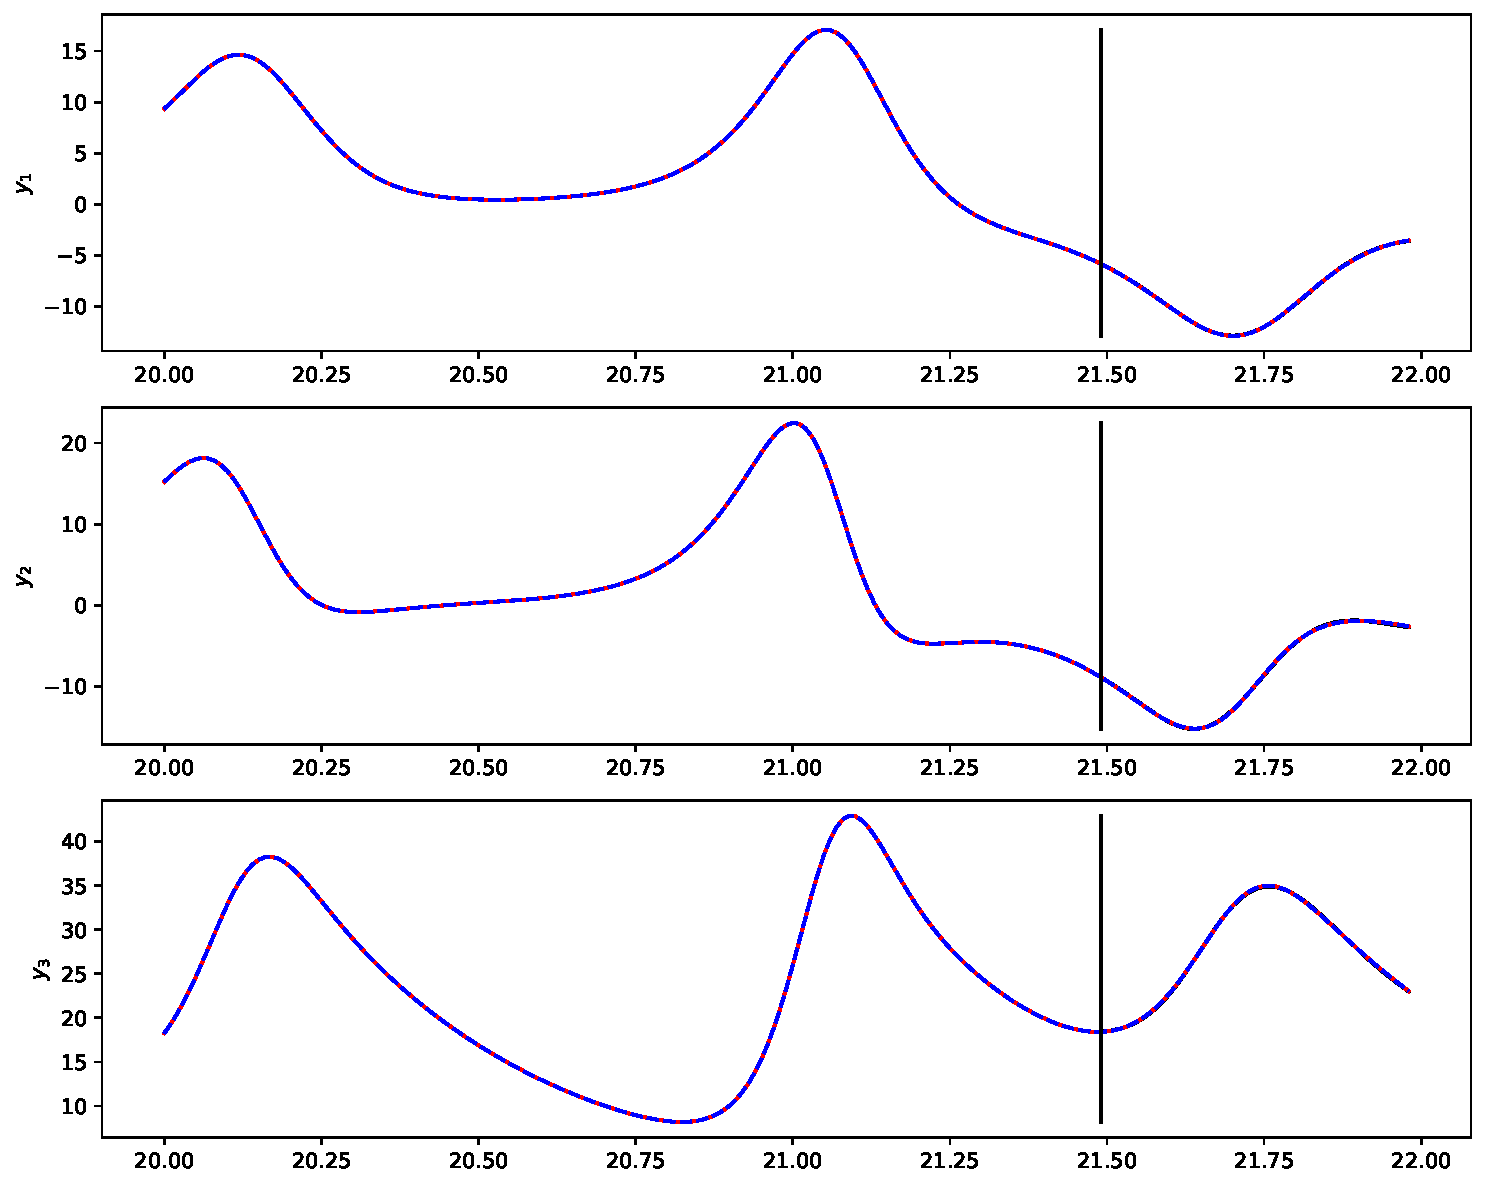
\includegraphics[width=1\textwidth]{lorenz_compare_w_mx_lag_150}
\caption{Comparison of ERDMD and all lags HODMD model against true trajectory for Lorenz-63 system.  The vertial bar indicates the maximum lag choice of $d=150$. The ERDMD algorithm converges to $l_{c}=\left\{1,149\right\}$.}
\label{fig:lorenz_compare_d_150}
\end{figure}

\begin{figure}[!h]
\centering
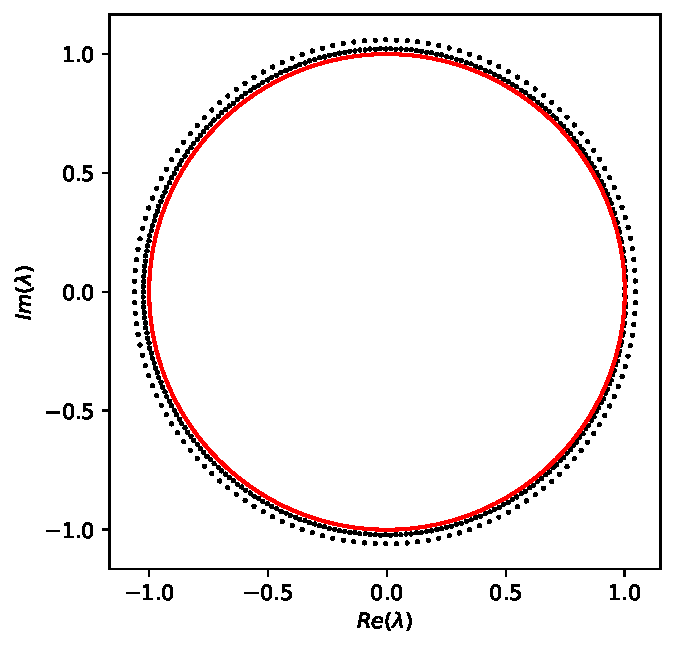
\includegraphics[width=.5\textwidth]{Lorenz_spectrum_w_mx_lag_149}
\caption{Spectrum of corresponding ERDMD Koopman operator.  The ERDMD algorithm converges to $l_{c}=\left\{1,149\right\}$.  The solid/red line is the unit circle, provided for comparison.}
\label{fig:lorenz_spectrum_d_150}
\end{figure}


By way of contrast though, if we set the maximum lag $d=100$, and build reconstructions for $21\leq t \leq 22$, we find that the ERDMD results differ  markedly in terms of the determined lags though ultimately not in terms of accuracy; see Figure \ref{fig:lorenz_compare_d_100}.  In this case, the ERDMD algorithm converges onto the lag choices 
$$
l_{c}=\left\{1,15, 26, 35, 45, 48, 68, 73, 97,99\right\}.
$$  By choosing a lag horizon which does not fully capture the approximate period of oscillation in the dynamics, we need significantly more information to accurately reconstruct the data, though still nowhere as much as the full HODMD model.  
\begin{figure}[!h]
\centering
\includegraphics[width=1\textwidth]{lorenz_compare_w_mx_lag_100}
\caption{Comparison of ERDMD and all lags HODMD model against true trajectory for Lorenz-63 system.  The ERDMD reconstruction is in solid black in the figure.  The vertial bar indicates the maximum lag choice of $d=100$. The ERDMD algorithm converges to $l_{c}=\left\{1,15, 26, 35, 45, 48, 68, 73, 97,99\right\}$.}
\label{fig:lorenz_compare_d_100}
\end{figure}
 
\begin{figure}[!h]
\centering
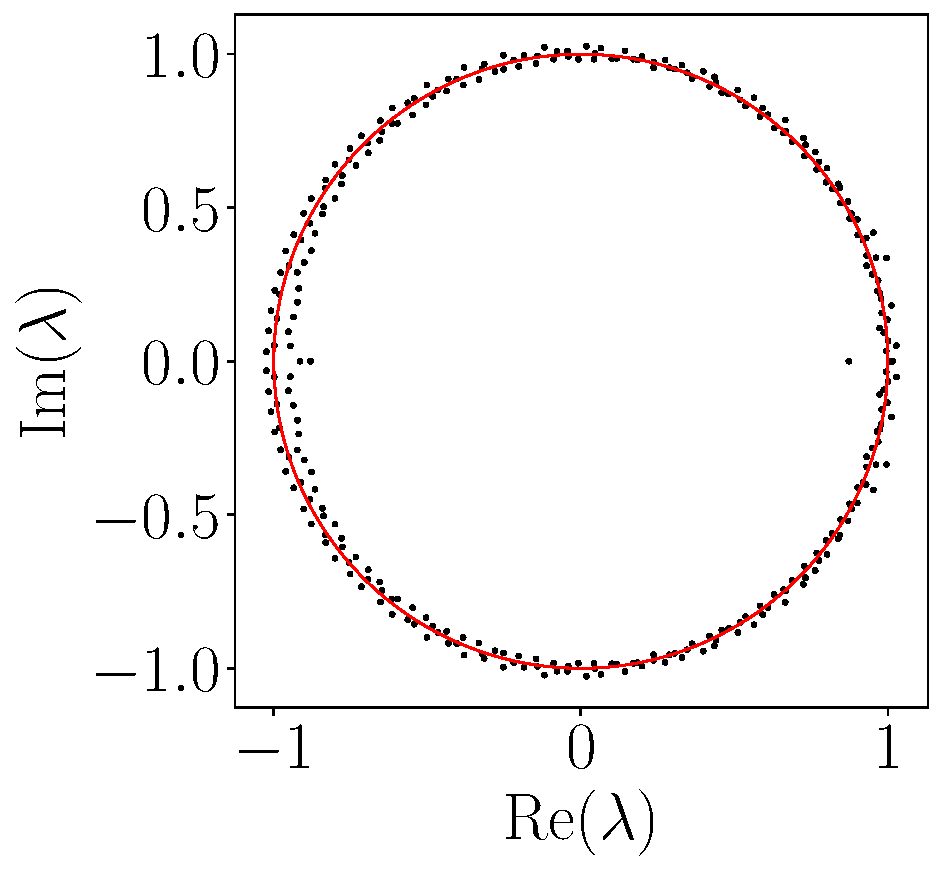
\includegraphics[width=.5\textwidth]{Lorenz_spectrum_w_mx_lag_99}
\caption{Spectrum of corresponding ERDMD Koopman operator.  The ERDMD algorithm converges to $l_{c}=\left\{1,15, 26, 35, 45, 48, 68, 73, 97,99\right\}$.  The solid/red line is the unit circle, provided for comparison.}
\label{fig:lorenz_spectrum_d_100}
\end{figure}
 
 
\subsection*{Kuramoto--Sivashinsky Equation}
To look at a more intricate and higher dimensional example, we now study the Kuramoto--Sivashinsky (KS) equation given by 
\[
u_{t} + u_{xx} + u_{xxxx} + uu_{x} = 0, ~ u(x+2L,t) = u(x,t).
\]
See \cite{robinson} for an extensive bibliography with regards to details and relavent proofs of facts used in this paper.  Introducing the rescalings
\[
\tilde{t} =\frac{t}{T}, ~ \tilde{x} = \frac{\pi}{L}x, ~ u = A\tilde{u},
\]
and taking the balances
\[
A = \frac{L}{\pi T}, ~ T = \left(\frac{L}{\pi}\right)^{2}, 
\]
we get the equivalent KS equation (dropping tildes for ease of reading)
\[
u_{t} + u_{xx} + \nu u_{xxxx} + uu_{x} = 0, ~ \nu = \left(\frac{\pi}{L}\right)^{2}.
\]
Looking at the linearized dispersion relationship $\omega(k) = k^{2} - \nu k^{4}$, we see that the $\nu$ parameter acts as a viscous damping term.  Thus, as the system size $L$ is increased, the effective viscosity is decreased, thereby allowing for more complex dynamics to emerge.  As is now well known, for $L$ sufficiently large, a fractional-dimensional-strange attractor forms which both produces intricate spatio-temporal dynamics while also allowing for a far simpler representation of said dynamics.  It is has been shown in many different works (see for example \cite{citanovic}) that $L=11$ generates a strange attractor with dimension between eight and nine, and that this is about the smallest value of $L$ which is guaranteed to generate chaotic dynamics.  We therefore set $L=11$ throughout the remainder of this section.  

To study ERDMD on the KS equation, we use KS data numerically generated by a pseudo-spectral in space and fourth-order exponential-differencing Runge-Kutta in time method \cite{kassam} of lines approach.  For the pseudo-spectral method, $K=128$ total modes are used giving an effective spatial mesh width of $2L/K = .172$, while the time step for the Runge-Kutta scheme is set to $\delta t = .25$.  After a burn in time of $t_{b}=10$, we generated a simulation of length $t_{f} = \left(L/\pi\right)^{4}\approx 160$ to allow for nonlinear effects to fully manifest.  This trajectory was then separated via a POD into space and time modes; see \cite{berkooz}.  Taking $N_{s}=12$ modes captured 98.6\% of the total energy.  

To study the ERDMD method, we choose $d=200$, which for $dt=.25$ corresponds to a lag time of $t=60$.  With this choice, the ERDMD method finds $l_{c}$ to be 
\[
l_{c}=\left\{1, 123, 141, 158\right\}.
\]
The results for reconstruction can be seen in Figure \ref{fig:ks_compare_d_200}, we where we look at times $10\leq t \leq 66$.  As can be seen, the ERDMD does quite well, though we note that if we look for longer reconstructions, errors do start to appear more rapidly for the ERDMD method than the full HODMD method.  
\begin{figure}[!h]
\centering
\includegraphics[width=1\textwidth]{ks_dynamics_compare}
\caption{Comparison of ERDMD and all lags HODMD model against true trajectory for the KS equation.  The vertial bar indicates the maximum lag choice of $d=200$. The ERDMD algorithm converges to $l_{c}=\left\{1, 123, 141, 158\right\}$.}
\label{fig:ks_compare_d_200}
\end{figure} 
 
\bibliographystyle{unsrt}
\bibliography{ionosphere_bib}
\end{document}
